\documentclass{article}

\usepackage[T1]{fontenc}

\usepackage{fancyhdr} % Required for custom headers
\usepackage{lastpage} % Required to determine the last page for the footer
\usepackage{extramarks} % Required for headers and footers
\usepackage[usenames,dvipsnames]{color} % Required for custom colors
\usepackage{graphicx} % Required to insert images
\usepackage{listings} % Required for insertion of code
\usepackage{courier} % Required for the courier font
\usepackage{lipsum} % Used for inserting dummy 'Lorem ipsum' text into the template
\usepackage{hyperref}
% Margins
\topmargin=-0.45in
\evensidemargin=0in
\oddsidemargin=0in
\textwidth=6.5in
\textheight=9.0in
\headsep=0.25in

\linespread{1.1} % Line spacing

% Set up the header and footer
\pagestyle{fancy}
\lhead{\hmwkAuthorName} % Top left header
\chead{\hmwkClass\ (\hmwkClassInstructor\ \hmwkClassTime): \hmwkTitle} % Top center head
\rhead{\firstxmark} % Top right header
\lfoot{\lastxmark} % Bottom left footer
\cfoot{} % Bottom center footer
\rfoot{Page\ \thepage\ of\ \protect\pageref{LastPage}} % Bottom right footer
\renewcommand\headrulewidth{0.4pt} % Size of the header rule
\renewcommand\footrulewidth{0.4pt} % Size of the footer rule

\setlength\parindent{0pt} % Removes all indentation from paragraphs

\usepackage{listings}
\usepackage{color}
\usepackage{hyperref}

\definecolor{dkgreen}{rgb}{0,0.6,0}
\definecolor{gray}{rgb}{0.5,0.5,0.5}
\definecolor{mauve}{rgb}{0.58,0,0.82}

\lstset{frame=tb,
  language=Java,
  aboveskip=3mm,
  belowskip=3mm,
  showstringspaces=false,
  columns=flexible,
  basicstyle={\small\ttfamily},
  numbers=none,
  numberstyle=\tiny\color{gray},
  keywordstyle=\color{blue},
  commentstyle=\color{dkgreen},
  stringstyle=\color{mauve},
  breaklines=true,
  breakatwhitespace=true
  tabsize=3
}

%----------------------------------------------------------------------------------------
%	DOCUMENT STRUCTURE COMMANDS
%	Skip this unless you know what you're doing
%----------------------------------------------------------------------------------------

% Header and footer for when a page split occurs within a problem environment
\newcommand{\enterProblemHeader}[1]{
\nobreak\extramarks{#1}{#1 continued on next page\ldots}\nobreak
\nobreak\extramarks{#1 (continued)}{#1 continued on next page\ldots}\nobreak
}

% Header and footer for when a page split occurs between problem environments
\newcommand{\exitProblemHeader}[1]{
\nobreak\extramarks{#1 (continued)}{#1 continued on next page\ldots}\nobreak
\nobreak\extramarks{#1}{}\nobreak
}




%----------------------------------------------------------------------------------------
%	NAME AND CLASS SECTION
%----------------------------------------------------------------------------------------

\newcommand{\hmwkTitle}{JML Plugin} % Assignment title
\newcommand{\hmwkDueDate}{Martedi,\ Aprile 15,\ 2015} % Due date
\newcommand{\hmwkClass}{Ingegneria del Software 1} % Course/class
\newcommand{\hmwkClassTime}{} % Class/lecture time
\newcommand{\hmwkClassInstructor}{Carlo Ghezzi} % Teacher/lecturer
\newcommand{\hmwkAuthorName}{} % Your name

%----------------------------------------------------------------------------------------
%	TITLE PAGE
%----------------------------------------------------------------------------------------

\title{
\vspace{2in}
\textmd{\textbf{\hmwkClass:\ \hmwkTitle}}\\
\normalsize\vspace{0.1in}\small{Due\ on\ \hmwkDueDate}\\
\vspace{0.1in}\large{\textit{\hmwkClassInstructor\ \hmwkClassTime}}
\vspace{3in}
}

\author{\textbf{\hmwkAuthorName}}
\date{} % Insert date here if you want it to appear below your name

%----------------------------------------------------------------------------------------

\begin{document}

\maketitle

%----------------------------------------------------------------------------------------
%	TABLE OF CONTENTS
%----------------------------------------------------------------------------------------

%\setcounter{tocdepth}{1} % Uncomment this line if you don't want subsections listed in the ToC

\newpage
\tableofcontents
\newpage



%----------------------------------------------------------------------------------------


%%%%%%%%%%%%%%%%%%%%%%%%%%%%%%%%%%
%OPEN JML
%%%%%%%%%%%%%%%%%%%%%%%%%%%%%%%%%%
% \section{Preliminaries}

% The Java Modeling Language (JML) is a language that enables logical
% assertions to be made about Java programs. The assertions are
% expressed as structured Java comments or Java annotations. Various
% tools can then read the JML information and do static checking,
% runtime checking, display for documentation, or other useful tasks.

% OpenJML is a suite of tools for editing, parsing, type-checking,
% verifying (static checking), and run-time checking Java programs that
% are annotated with JML statements that describe what the program's
% methods are supposed to do. JML annotations state preconditions,
% postconditions, invariants and the like about a method or class;
% OpenJML is a tool that will then check that the implementation does
% indeed satisfy those specifications by translating JML specifications into
% SMTLIB format and passing the proof problems implied by the Java+JML
% program to backend
% \href{http://en.wikipedia.org/wiki/Satisfiability_Modulo_Theories}{SMT solvers}.

% OpenJML is built on the OpenJDK framework for
% Java. It is current with Java 1.7u6. 


% \subsection{Documentation}
% The OpenJML user guide is available
% \href{http://jmlspecs.sourceforge.net/OpenJMLUserGuide.pdf}{here}, also
% in form of an \href{http://jmlspecs.sourceforge.net/onlinemanual.shtml} {online user guide}. 

% \subsection{Install OpenJML}
% You can install last OpenJML release by using the following update site from within Eclipse:

% \url{http://jmlspecs.sourceforge.net/openjml-updatesite}

% Perform following steps:
% \begin{itemize}
% \item To to Help > Install New Software\\
% 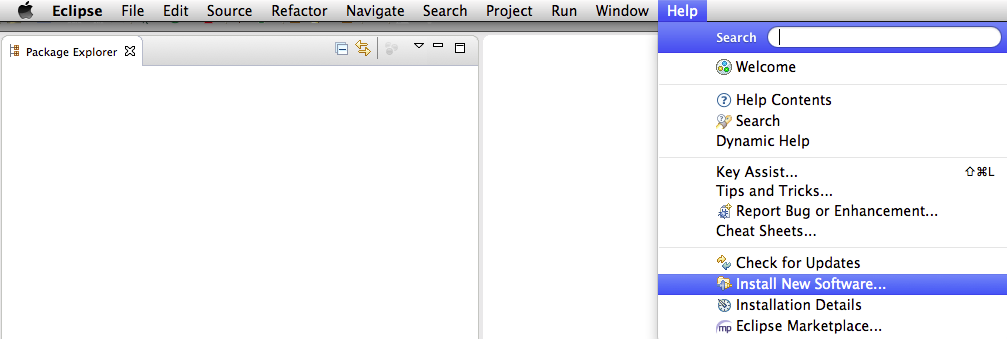
\includegraphics[scale=0.4]{Photos/1.png}
% \item Copy the above URL into the topmost textbox
% \item Click on add and give it a name
% \item After clicking OK, the list below should contain ''OpenJML``
% \item Check it\\
% 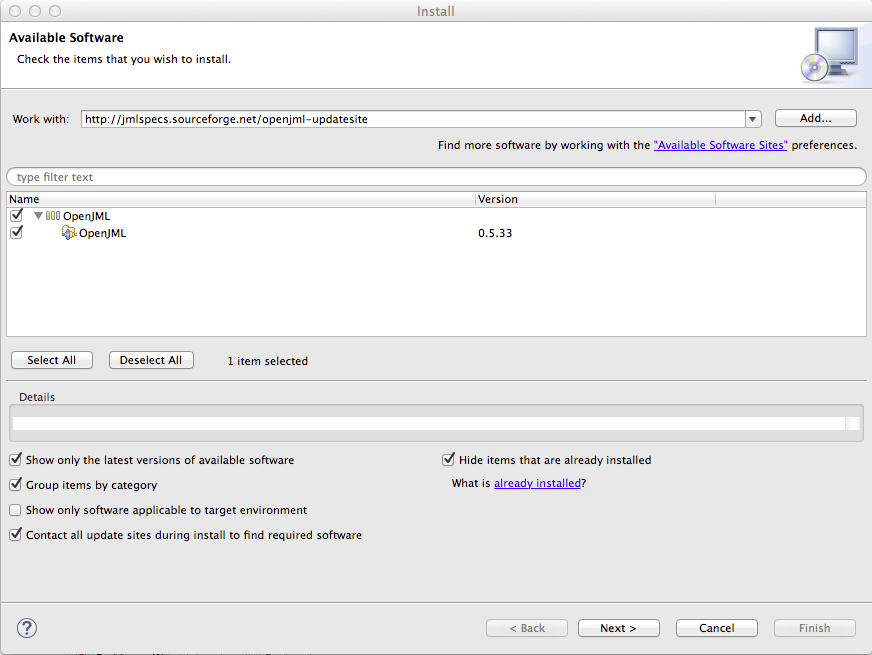
\includegraphics[scale=0.4]{Photos/2.png}
% \item Click Next, Next, Accept, Finish\\
% 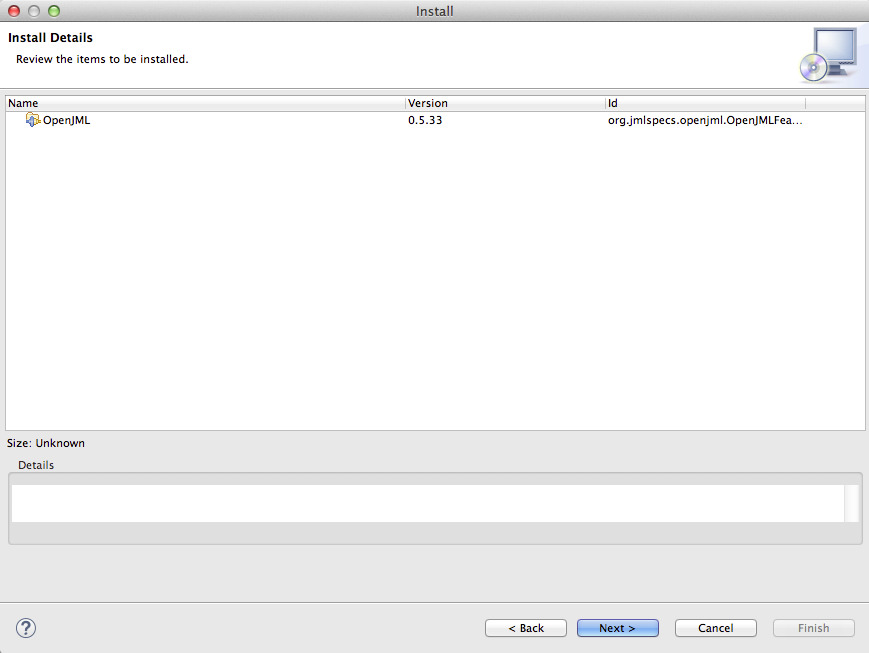
\includegraphics[scale=0.4]{Photos/3.png}\\
% 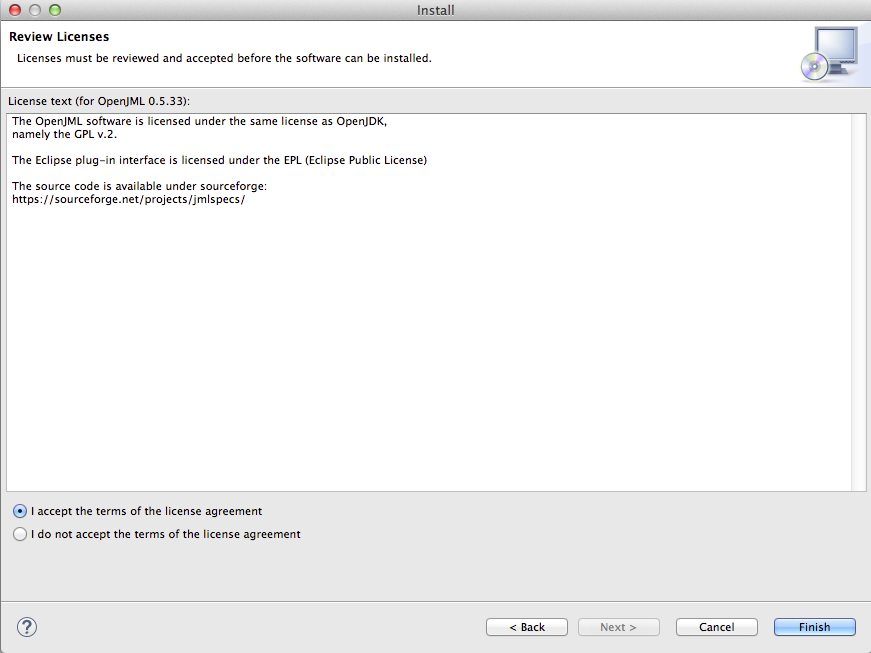
\includegraphics[scale=0.4]{Photos/4.png}\\
% 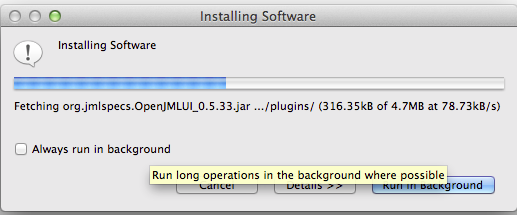
\includegraphics[scale=0.4]{Photos/5.png}\\
% \item You need to accept that you are installing unsigned software\\
% 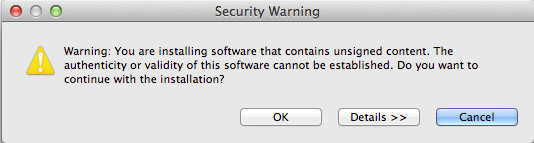
\includegraphics[scale=0.4]{Photos/6.png}
% \item Restart Eclipse\\
% 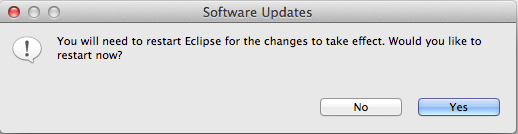
\includegraphics[scale=0.4]{Photos/7.png}
% \end{itemize}

% To enable JML functionality, you will need to do these additional
% tasks:
% \begin{itemize}
% \item For each project of interest, select the project name in the Package Explorer View and then the JML >> Enable JML for project menu action.
% \item On the OpenJML Solvers preference page, select a default solver and enter the path to the solver executable.
% \item On the OpenJML preference page, select the 'Skip Purity Check' option.
% \end{itemize}


% \subsection{Features}

% \subsubsection{Menubar and toolbar items}

% The Menubar and toolbar contain these additional items:
% The JML menubar entry with its submenu items.
% \begin{itemize}
% \item A toolbar item marked by the JML logo (a yellow coffee cup), which initiates type-checking of a Java or JML file.
% \item A toolbar item marked ESC, which initiates static checking of selected files, classes or methods.
% \item A toolbar item marked RAC, which initiates compilation for runtime
% assertion checking.
% \end{itemize}

% The JML sub-menu items are described in detail in the Help
% documentation. Note that the same menu actions are available from the
% 'JML' item on the main menubar, from context menus in Package
% Explorer, Navigator, and Outline (and perhaps other) Views. The menu
% actions provide the following groups of functionality:
% \begin{itemize}
% \item enabling and disabling JML on a project
% \item typechecking all or a selected set of files
% \item static checking all or a selected set of files, or individual methods
% \item applying runtime assertion compilation to all or a selected set of files
% \item adding or removing files from the set of files that are automatically RAC-compiled
% \item viewing and editing the sourcepath and specspath
% \item showing counterexample model information generated by a (failed) attempt to validate a method
% \item showing the composite (including inherited) specs for a method
% \item opening an editor on the .jml file corresponding to a .java file
% cleaning up errant JML problem markers
% \end{itemize}

% \subsubsection{JML Nature and automatic building}

% By enabling JML for a project (select a project and then activate the 'Enable JML' menu item), you add the Eclipse JML Nature to the project (along with the Java Nature for the project). When JML is enabled, the project icon in the Package Explorer and other Views is decorated with the JML logo (the yellow coffee cup) in its upper right. More importantly, OpenJML type-checking of files is automatically performed whenever the file is built by the Java compiler. Thus if you have 'Build Automatically' enabled for the project, then any file is compiled whenever it is saved; if the JML Nature is enabled, the file will also be type-checked by OpenJML whenever it is saved. Note that OpenJML only operates on the saved version of the file, not on the content of an unsaved (dirty) editor.

% You can also enable automatic Runtime Assertion Compilation or Extended Static Checking for files upon saving. These are not enabled by default. More detail is provided about the appropriate use of these features in the Help documentation.

% \subsubsection{JML problem markers}

% The OpenJML plugin shows problems reported by OpenJML as Eclipse
% Problem Markers, with all the functcionality such markers have in
% Eclipse:
% \begin{itemize}
% \item The markers are displayed in editors
% \item The appearance of the markers can be customized using the
%   options on the Preference page at General>>Editors>>Text
%   editors>>Annotations. You can turn the markers on and off in either
%   the left or right rulers and change the color and style (highlight
%   or squigglies) of the marker. 
% \item The OpenJML errors and warnings are listed in the Problem
%   View. The Problems have a category (JML) enabling the Problem View to customize
% when they are to be displayed in the View's list.
% \end{itemize}


% \subsubsection{JML Console}

% OpenJML contributes an additional kind of Console (the JML Console) to Eclipse. Various textual information will be written to the console as OpenJML operations are executed. The amount of information can be controlled by options on the OpenJML Preferences page. The information is in large part the same information that is produced by the OpenJML command-line tool, augmented with some information about the operation of the plugin itself.

% \subsubsection{File association for .jml files and the Java editor}

% The plugin creates a new content type for .jml files and associates it with the Java editor. So you can double-click a .jml file to open an editor and all the Java editing capability is available for .jml files.
% However, since we are using a standard Java editor, there is no special knowledge of JML syntax. It is a future work item to extend the Java editor to be JML-aware. Note that the Eclipse Java compiler is still active, even when the OpenJML compiler is present to do JML checkin.

% Consequently the Java compiler will issue errors about some legitimate JML features:
% \begin{itemize}
% \item JML files may contain class declarations even though the suffix is not .jml.
% \item Method declarations in JML files do not have bodies (even though they are not abstract).
% \item Final field declarations in JML files are not initialized.
% \end{itemize}

% \subsubsection{Preferences}

% The OpenJML plugin contributes a typical Preferences Page to the Eclipse preferences menu. It is accessed through the top-level 'OpenJML' item in the Preferences outline.
% There are two preference pages -- a main one with most of the
% individual options and a subsidiary page on which paths to solvers are
% set. The subsidiary page is seen by opening up the twisty by the
% OpenJML item in the Preferences outline.

% The Preference options correspond to the options available in the command-line tool, discussed \href{http://jmlspecs.sourceforge.net/commandline.shtml}{here}. There are a few points to note:
% \begin{itemize}
% \item One must specify the solver to use for ESC on the Solvers page, as well as the paths to the executables of any solver intended to be used.
% \item The command-line tool uses option settings taken from a
% openjml.properties file. An Eclipse plug-in has its own, separate
% properties persistence mechanism. So the Eclipse plugin does not use
% the openjml.properties file. However, there is a button on the
% preferences page: clicking it will set the preferences by loading them
% from the openjml.properties page. This can be used as a one-time
% initialization of the Eclipse preferences.
% \end{itemize}

% % \subsubsection{Commands and key associations}

% % All actions (i.e., responses to menu selections) contributed by the OpenJML plugin are associated with Eclipse Commands. Thus they appear in the list of commands on the General>>Keys preference page and can have keyboard bindings associated with them.

% % \subsubsection{Eclipse help}

% % Conventional Eclipse Help about the OpenJML plugin is available from Eclipse's Help>>Help Contents menu item.

% \section{Usage}

% Type-checking

% \begin{lstlisting}
% public class A {

%   //@ ensures \result == true;
%   public void m() {}

% }
% \end{lstlisting}

% Static checking

% \begin{lstlisting}
% public class B {

%   static int j,k;

%   //@ requires i >= 0;
%   //@ modifies j;
%   //@ ensures j == i;
%   public static void setj(int i) {
%     k = i;
%   }

%   //@ ensures j == 1;
%   public static void main(String[] args) {
%     setj(3);
%   }

% }
% \end{lstlisting}


% Runtime assertion checking





%%%%%%%%%%%%%%%%%%%%%%%%%%%%%%%%%%
% COFOJA
%%%%%%%%%%%%%%%%%%%%%%%%%%%%%%%%%%

\section{Preliminaries}

The Java Modeling Language (JML) is a language that enables logical
assertions to be made about Java programs. The assertions are
expressed as structured Java comments or Java annotations. Various
tools can then read the JML information and do static checking,
runtime checking, display for documentation, or other useful tasks.

Contracts for Java, or Cofoja for short, is a contract programming
framework and test tool for Java, which uses annotation processing and
bytecode instrumentation to provide run-time checking. (In particular,
this is not a static analysis tool.) 

\subsection{Documentation}

Documentation can be found in the
\href{https://github.com/nhatminhle/cofoja}{\textbf{Readme file on the
    GitHub page}}.

\subsection{Add Cofoja to your Eclipse project}
\label{subsec-add}

 Perform following steps:
 \begin{itemize}
\item Make sure you are running Eclipse with JDK 1.7u67 (not JRE!)
\item Start a new Java project (or import an existing one)
\item Create a new lib folder 
\item Pre-built JAR files are available on the GitHub
\href{https://github.com/nhatminhle/cofoja/releases}{\textbf{release
    page}}. Download them.
\item Place the files in the lib folder
\item Add the .jar files to the build path by right-clicking the .jar
  files: Build Path>> Add to Build Path
\item In order to enable Annotation Processing in Eclipse we will 
need to configure the project preferences. Right click the project: 
Properties>>Java Compiler>>Annotation Processing>>Enable 
project specific settings
\item The annotation processor will need to be configured with 
the following parameters (Use the New… button):
  \begin{description}
\item - Key: com.google.java.contract.classpath \\
Value:\%PROJECT.DIR\%/lib/cofoja.contracts-1.2-20140817.jar
\item - Key: com.google.java.contract.sourcepath \\
Value:\%PROJECT.DIR\%/src
\item - Key: com.google.java.contract.classoutput \\
Value: \%PROJECT.DIR\%/bin\\
In cases where there are multiple folders use the ";" delimiter in Windows or ":" in Unix to separate the 
values.\\
 \end{description}
\item Next the location of the annotation factory has to be defined. Under Java 
Compiler>>Annotation Processing>>Factory Path, you should enable the specific project 
settings and add the cofoja.contracts-1.2-20140817.jar file. 

 \end{itemize}

\subsection{Cofoja Quick Reference}


\textbf{Annotations}\\

All annotations reside in the com.google.java.contract package.

\begin{tabular}{|c|c|c|}
\hline
Annotation&             Checked on&                     Inheritance\\
\hline
@Invariant&              Object entry and exit&       And\\
\hline
@Requires&              Entry&                                Or\\
\hline
@Ensures&               Normal exit&                      And\\
\hline
@ThrowEnsures&	Abnormal exit&                   And\\
\hline
\end{tabular}\\

\textbf{Keywords}\\

\begin{tabular}{|c|c|c|}
\hline
Keyword&                May appear in&                         Description\\
\hline
old&                        @Ensures, @ThrowEnsures&         Value on method entry\\
\hline
result&                    @Ensures&                              Value to be returned\\
\hline
signal&                   @ThrowEnsures&                    Exception thrown\\
\hline
\end{tabular}

 \section{Usage}

Here we assume you have followed instruction and created a project,
like shown in Sec.~\ref{subsec-add}.

\subsection{Annotations}

In Cofoja, contracts are written as Java code within quoted strings, embedded in annotations. E.g., @Requires("x < 100") states that x must be less than 100. Any Java expression, except anonymous classes, may be used, provided the string is properly escaped.

An annotation binds a contract to a code element: either a method or a type. Cofoja defines three main annotation types, which live in the com.google.java.contract package:

@Requires for method preconditions;\\
@Ensures for method postconditions;\\
@Invariant for class and interface invariants;\\

Contract annotations work on both classes and interfaces. For convenience, arrays of quoted expressions are accepted, and behave as if the components were separated by \&\&. E.g., @Ensures({ "x > 0", "x < 50" }) is equivalent to @Ensures("x > 0 \&\& x < 50").

\subsection{Method contracts}

A method may have preconditions and postconditions attached to
it. Together, they specify the contract between caller and callee: if
the precondition is satisfied on entry of the method, then the caller
may assume the postcondition on exit. The precondition is what the
callee demands of the caller, and in return the caller expects the
postcondition to hold after the call.

For example lets perform the following steps:
 \begin{itemize}
\item Create package "src"
\item Create a class "Main" inside package "src"
\item Write the static method "sqrt" and its specification, which states
that for any non-negative double x given, sqrt will return a
non-negative result. 
\begin{lstlisting}
package src;
import com.google.java.contract.Ensures;
import com.google.java.contract.Requires;

public class Main {

	@Requires("x >= 0")
	@Ensures("result >= 0")
	public static double sqrt(double x)
	{
		return 0;
		
	}
	
}
\end{lstlisting}
\end{itemize}

As shown in this example, a precondition may access parameter values; in fact, preconditions and postconditions are evaluated in the context of the method they are bound to. More precisely, each annotation behaves as if it were a method, with the same arguments and in the same scope as the qualified method. In terms of scoping, the previous code is equivalent to the following:

\begin{lstlisting}

static void sqrt_Requires(double x) {
  assert x >= 0;
}
static void sqrt_Ensures(double result) {
  assert result >= 0;
}
static double sqrt(double x);

\end{lstlisting}

In addition, postconditions may contain a few extensions:

As we have seen, they may refer to the returned value, using the "result" keyword.
Within a postcondition, "old" is a keyword which is followed by a
single parenthesized expression, such that old (x) evaluates to the
value of x on entry of the method invocation. 
An old expression is evaluated in the same context as preconditions
and has access to the same things, including parameter values. 

Given this, lets write a more complete specification of sqrt:

\begin{lstlisting}
package src;
import com.google.java.contract.Ensures;
import com.google.java.contract.Requires;
import java.lang.Math;

public class Main {

	private static double EPS = 0.0001;
	@Requires("x >= 0")
	@Ensures({ "result >= 0", "Math.abs(x - result * result) < EPS" })
	public static double sqrt(double x){
		return 0;	
	}
}


\end{lstlisting}

At run time, when contracts are enabled, preconditions and postconditions translate to checks on entry and exit, respectively, of the method. A failure results in a PreconditionError or PostconditionError being thrown, depending on the origin: failure to meet a precondition means that the method was called incorrectly, whereas an unsatisfied postcondition points to a bug in the implementation of the method itself.

To demonstrate this perform the following steps:

\begin{itemize}
\item Create package "test"
\item Create JUnit test "TestMain"
\item Put src.Main in Class under test field\\
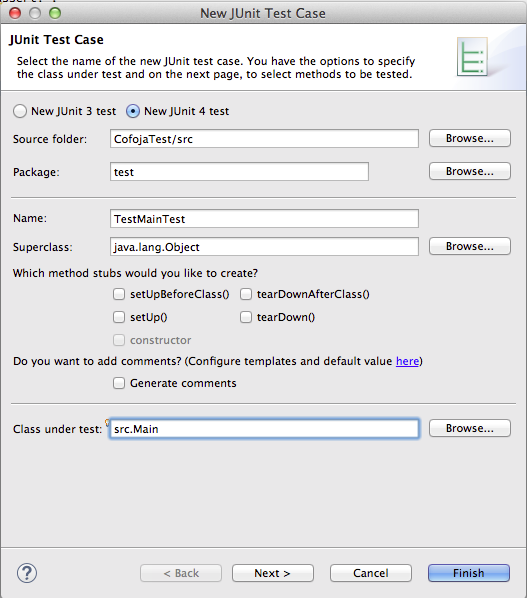
\includegraphics[scale=0.4]{Photos/8.png}\\
\item Write the test:
\begin{lstlisting}
package test;

import static org.junit.Assert.*;
import org.junit.Test;
import src.*;

public class TestMain {
	@Test
	public void test() {
		Main.sqrt(-1);
	}
}

\end{lstlisting}
\item Right click on the TestMain file in the package explorer and
  choose Run As>>Run Configurations...
\item Double click on JUnit to create new running configuration
\item Rename TestMain to TestJML in the name field
\item Put -javaagent:lib/cofoja.contracts-1.2-20140817.jar into VM
  arguments under the Arguments tab
\item Click Run\\
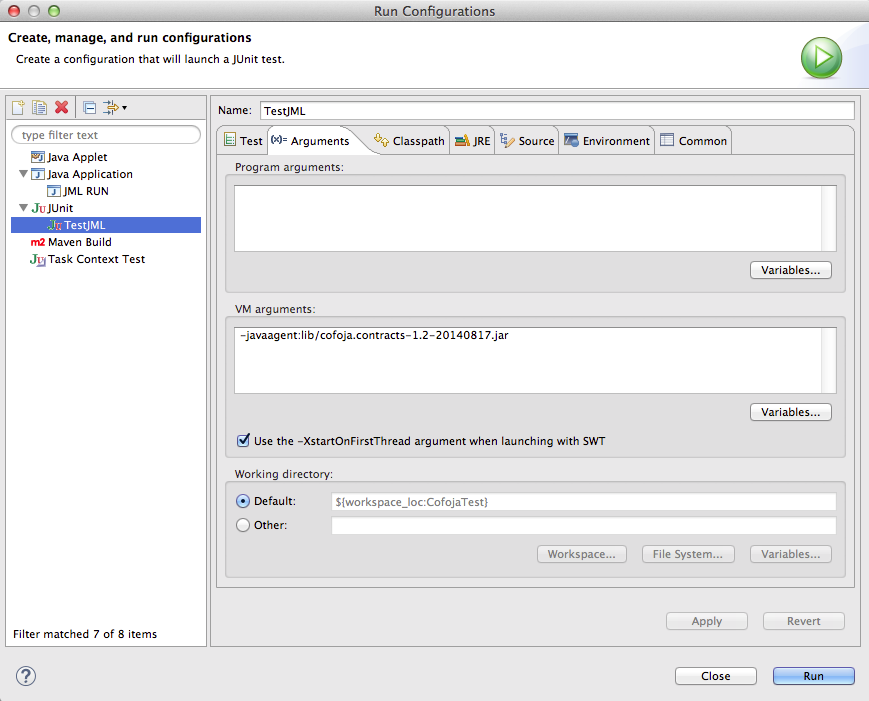
\includegraphics[scale=0.4]{Photos/11.png}\\
\item You obtain a failure trace that states that the precondition is
  violated. This is expected since we called sqrt with argument -1.\\
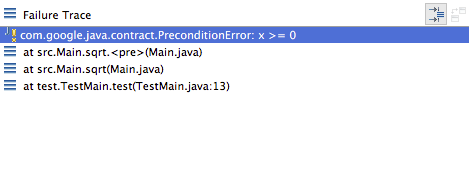
\includegraphics[scale=0.7]{Photos/9.png}\\
\item Now, lets change the test to:
\begin{lstlisting}
@Test
public void test() {
	Main.sqrt(4);
}
\end{lstlisting}
\item We get a different kind of error; now postcondition is violated
  since $|4-0\cdot 0|$ is not less than $EPS=0.0001$.\\
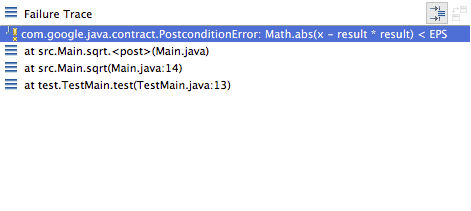
\includegraphics[scale=0.7]{Photos/10.png}\\
\item Finally we change the implementation of sqrt method in class Main:
\begin{lstlisting}

public static double sqrt(double x)
{
	return Math.sqrt(x);
}

\end{lstlisting}
\item And we import the java.lang.Math package
\item If we execute the test again, we should not see any errors
\end{itemize}



\subsection{Class and interface contracts}

A class or interface may have associated invariants. Instead of specifying a contract between a caller and a callee, those invariants describe the state of a valid object of the qualified type. Calling methods on an object may cause it to change; invariants guarantee that after any such change, the object remains in a consistent state.

Of course, internal operations are allowed to muck around and temporarily invalidate invariants to do their job, but they agree to eventually put everything back into their proper places. Intuitively, any operation made against this is considered internal and does not need to obey the invariants. Only method invocations on other variables do.

In Cofoja, when contracts are enabled, invariants are checked on entry and exit of method calls on objects not already in the call stack (including this). Failure results in an InvariantError exception and indicates that the guilty method has left the object in an inconsistent state.

\subsection{Inheritance}

Contracts apply to all objects of the associated type, including any instances of derived classes: all implementations of a contracted interface must honor the interface contracts, all children of a class must honor the contracts of their parent.

In addition, derived types may refine those contracts by adding their own preconditions, postconditions and invariants to the mix. However, they cannot replace the inherited contracts, only augment them according to the following subtyping rules.

Preconditions may be weakened, i.e., methods may be overriden with implementations that accept a wider range of inputs. Callers that access the object through a superclass or interface need only establish the parent contracts. In Cofoja, a method checks that either its inherited or its own preconditions are satisfied.

Postconditions may be strengthened, i.e., methods may be overriden with implementations that produce a smaller range of outputs. Callers that access the object through a superclass or interface expect at least the parent contracts. In Cofoja, a method checks both its inherited and its own postconditions.

Invariants may be strengthened, i.e., classes and interfaces may be derived to restrict the set of valid states. An object must qualify as a consistent value of any of its superclasses or interfaces. In Cofoja, a type asserts both its inherited and its own invariants.



\end{document}




